\documentclass[german]{latteachCD}
\usepackage{mdframed}
\usepackage{amsmath}
\usepackage{amsfonts}
\usepackage{amssymb}
\usepackage{fdsymbol}
%\usepackage{wasysym}
%\usepackage{stmaryrd}
%\usepackage{fixltx2e}
%\usepackage{enumitem}
%\usepackage{extarrows}
%\newcommand{\abs}[1]{\lvert#1\rvert}

\usepackage{tikz}
\usetikzlibrary{arrows,automata,positioning,shapes,calc,decorations.pathmorphing,matrix}

\tikzstyle{automaton}=[->, >=stealth', initial text=, auto, node distance=20mm, bend angle=20, semithick, x=20mm, y=20mm]
\tikzset{
  every state/.style={
    inner sep=0pt,
    minimum size=8mm
  },
  small state/.style={
      state,
      minimum size=3mm
  },
  ellipse state/.style={
    draw,
    shape=ellipse,
    minimum width=20mm,
    minimum height=12.36mm,
    text width=14.5mm,
    inner sep=0mm,
    path picture={
      \draw (path picture bounding box.east) ellipse [x radius=9mm, y radius=9mm];
    }
  },
  accepting ellipse state/.style={
    ellipse state,
    path picture={
      \clip (path picture bounding box.east) ellipse [x radius=9.4mm, y radius=9.4mm];
      \draw[double] (path picture bounding box.east) ellipse [x radius=9mm, y radius=9mm];
      \draw[double] (path picture bounding box.center) ellipse [x radius=10mm, y radius=6.18mm];
    }
  }
}


\newcommand{\cKeps}{\ensuremath\mathcal{M}_{\varepsilon}}
\newcommand{\cLeps}{\ensuremath L_{\varepsilon}}
\newcommand{\cK}{\ensuremath\mathcal{M}}
\newcommand{\cL}{\ensuremath L}

%%%%%%%%%%%%%%%%%%%%%%%%%%%%%%%%%%%%%%%%%%%%%%%%%%%%%%%%%%%%%%%%%%%%%%%%%%%%%%%%%%%%%%%%%%%%

\usepackage{xspace}

\author{~}
\term{Wintersemester 2017/18}
\title{\Large 9.\@ Übungsblatt}
\course{\LARGE Formale Systeme}

\usepackage{csquotes}
\usepackage{booktabs}
\usepackage{amsmath}
\usepackage{amsfonts}
\usepackage{amssymb}
\usepackage{mathtools}
\usepackage{wasysym}
\usepackage{stmaryrd}
\usepackage{enumitem}
\usepackage{tikz}
\usepackage{makecmds}

\renewcommand{\epsilon}{\varepsilon}
\renewcommand{\phi}{\varphi}
\renewcommand{\rho}{\varrho}
\renewcommand{\theta}{\vartheta}
\newcommand{\tuple}[1]{\langle{#1}\rangle} 

\newcommand{\size}[1]{\ensuremath{\lvert #1\rvert}}
\newcommand{\gdw}{\mathrel{\mathrm{gdw.}}}
\newcommand{\falls}{\mathrel{\mathrm{falls}}}

\provideenvironment{solution}{\textbf{Lösung}:}{}
\usepackage{comment}

\usepackage{etex,etoolbox}

\DeclareRobustCommand{\NN}{\ensuremath{\mathbb{N}}}

\newbool{Baader}
\newbool{Kroetzsch}
\booltrue{Kroetzsch}

\DeclareMathOperator{\Var}{Var}
\ifbool{Baader}{%
  \DeclareMathOperator{\Unt}{Unt}
  \DeclareMathOperator{\Res}{Res}
}{}
\ifbool{Kroetzsch}{%
  \DeclareMathOperator{\Unt}{Sub}
  \DeclareMathOperator{\Res}{Res}
  \usepackage{multicol}         % for resolution
}{}

\excludecomment{solution}

\begin{document}

\maketitle

\begin{center}
\begin{mdframed}
  \renewcommand{\theexercise}{zur Selbstkontrolle
  (diese werden in den Übungen nicht besprochen)}
  
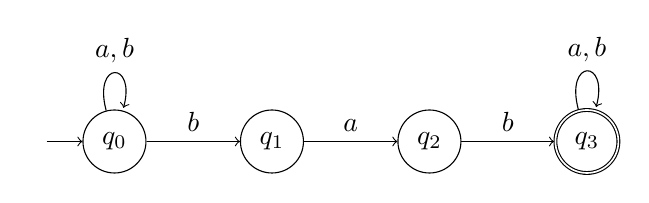
\begin{tikzpicture}[node distance=2cm, auto]
   \node[state,initial,initial text= ] (q0) {$q_0$};
   \node[state] (q1) [right of=q0] {$q_1$};
   \node[state] (q2) [right of=q1] {$q_2$};
   \node[state, accepting] (q3) [right of=q2] {$q_3$};

\path[->] (q0) edge [loop above] node {$a,b$} ()
               edge              node {$b$} (q1)
          (q1) edge              node {$a$} (q2)
          (q2) edge              node {$b$} (q3)
          (q3) edge [loop above] node {$a,b$} ()
;
\end{tikzpicture}

%  {\bfseries Hinweis:} Die Aufgaben *) und **)
%  dienen der Selbstkontrolle und werden in der
%  Übung nicht besprochen.
\end{mdframed}
\end{center}

%\vspace*{0.5cm}
%{\bf{Anmerkung}}\\
%Mit der 9. \"Ubung ist in den verschiedenen \"Ubungsgruppen abzusichern, dass alle bisher aus Zeitgr\"unden noch nicht besprochenen Aufgaben der \"Ubungsbl\"atter 1 bis 8 abgearbeitet sind.

\setcounter{exercise}{0}


\begin{exercise}
Gegeben sei die Sprache $L=\{w\in \Sigma^*\;|\;|w|_a+|w|_b=|w|_c\}$ \"uber dem Alphabet $\Sigma =\{a,b,c\}$, wobei $|w|_a$ der Anzahl der Vorkommen von $a$ in $w$ entspricht.
 \begin{enumerate}
    \item[a)] Entwerfen Sie einen Kellerautomaten $\mathcal{M}$ mit $L(\mathcal{M})=L$, der mittels Finalzustand akzeptiert.
    \item[b)] Welcher andere Akzeptanzbegriff f\"ur Kellerautomaten ist laut Anmerkung in der Vorlesung auch m\"oglich?
    \item[c)] Wann ist eine Sprache deterministisch kontextfrei? Ist $L$ deterministisch kontextfrei?
 \end{enumerate}
\end{exercise}


\begin{exercise}
Welche der folgenden Aussagen sind wahr und welche nicht? Begr"unden Sie Ihre
Antworten -- dabei d"urfen Sie den gesamten Stoff und alle Resultate
der Vorlesung und "Ubung verwenden.
 \begin{enumerate}
    \item[a)] Es gibt eine Sprache, die von einem nichtdeterministischen Kellerautomaten erkannt wird, nicht aber von einem deterministischen Kellerautomaten.
    \item[b)] Mithilfe des Pumping-Lemmas f\"ur kontextfreie Sprachen kann
              bewiesen werden, dass eine Sprache $L$ kontextfrei ist. 
    \item[c)] F\"ur eine beliebige Sprache $L$ gilt: $L$ ist regul\"ar, wenn es eine nat\"urliche Zahl $n_0\ge 1$ gibt, so dass sich jedes Wort $w\in L$ mit $|w|\ge n_0$ zerlegen l\"asst in $w=xyz$ mit $y\not = \varepsilon, xy^kz\in L$ f\"ur alle $k\ge 0$.
 \end{enumerate}
\end{exercise}



%%%%%%%%%%%%%%%%%%%%%%%%%%%

\begin{exercise}

Entwerfen Sie einen (nichtdeterministischen) PDA~$\cKeps$ 
mit Akzeptanz durch leeren Keller, dessen akzeptierte Sprache
$\cLeps(\cKeps)$ mit der Sprache
\[ 
  L \, = \, \bigl\{ w \in \{a,b,c\}^* : w = w^R \bigr\}
\]
\"ubereinstimmt, und begr\"unden Sie die Korrektheit. Hierbei bezeichnet $w^R$ das
Wort $w$ in umgekehrter Zeichenfolge.
%
%Wenden Sie dann die in der Vorlesung  besprochene
%Transformation an, die $\cKeps$
Transformieren Sie $\cKeps$ in einen \"aquivalenten 
(nichtdeterministischen) PDA~$\cK_F$ mit Akzeptanz 
\"uber Endzust\"ande.
% transformiert.
Geben Sie jeweils einen akzeptierenden Lauf von
$\cKeps$ und  $\cK_F$ f\"ur die W\"orter $ababa$ 
und $abba$ an.

\end{exercise}


\begin{exercise}
	
Zeigen Sie, dass die Sprache
$L \, = \, \bigl\{ w \$ w^R : w \in \{a,b\}^* \bigr\}$
\"uber dem Alphabet $\Sigma = \{a,b,\$\}$ deterministisch  
kontextfrei ist. Hierbei bezeichnet $w^R$ das
erneut das Wort $w$ in umgekehrter Zeichenfolge.

\end{exercise}

%\input{pool/baier/741}

%%%%%%%%%%%%%%%%%%%%%%%%%%%

\end{document}
